\section{TransforMMer}

To solve the indicated open problems, \textit{TransforMMer} enables the transformation of virtually any input dataset (single- or multi-model) to a required output multi-model dataset. 

\subsection{Sample Scenario}
Let us consider a simple scenario to demonstrate the purpose and advantages of \textit{TransforMMer}. We want to use the subset of the Yelp Open Dataset\footnotei{\url{https://www.yelp.com/dataset}}{,} namely the data that describes businesses, tips, and users, represented using the JSON format as depicted in Fig.~\pRef{figure:data-initial}. 

\begin{figure}[ht]
    \centering
    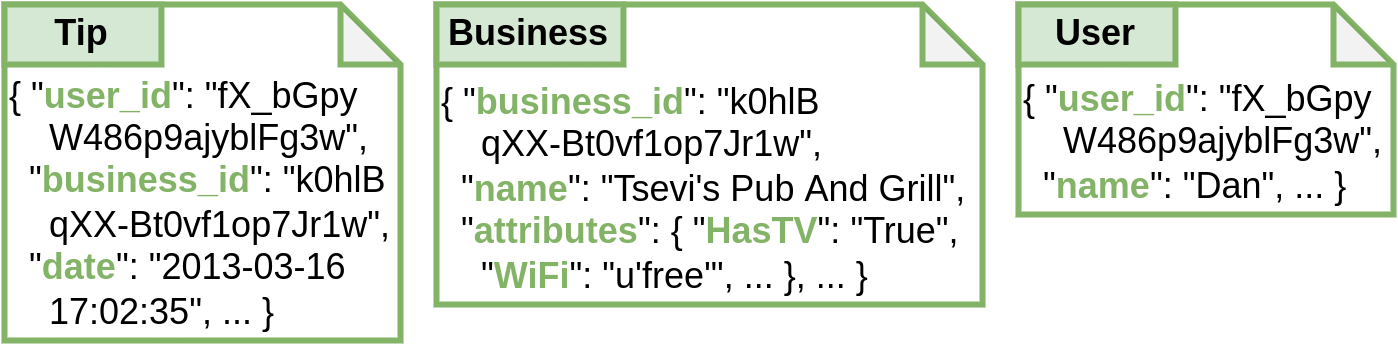
\includegraphics[width=0.8\textwidth]{papers/edbt_2025/figures/data-initial.png}
    \caption{Input Yelp dataset in the document model}
    \pLabel{figure:data-initial}
\end{figure}

We want to transform the data into a combination of the relational and graph models, e.g., the one depicted in Fig.~\pRef{figure:data-final}.

\begin{figure}[ht]
    \centering
    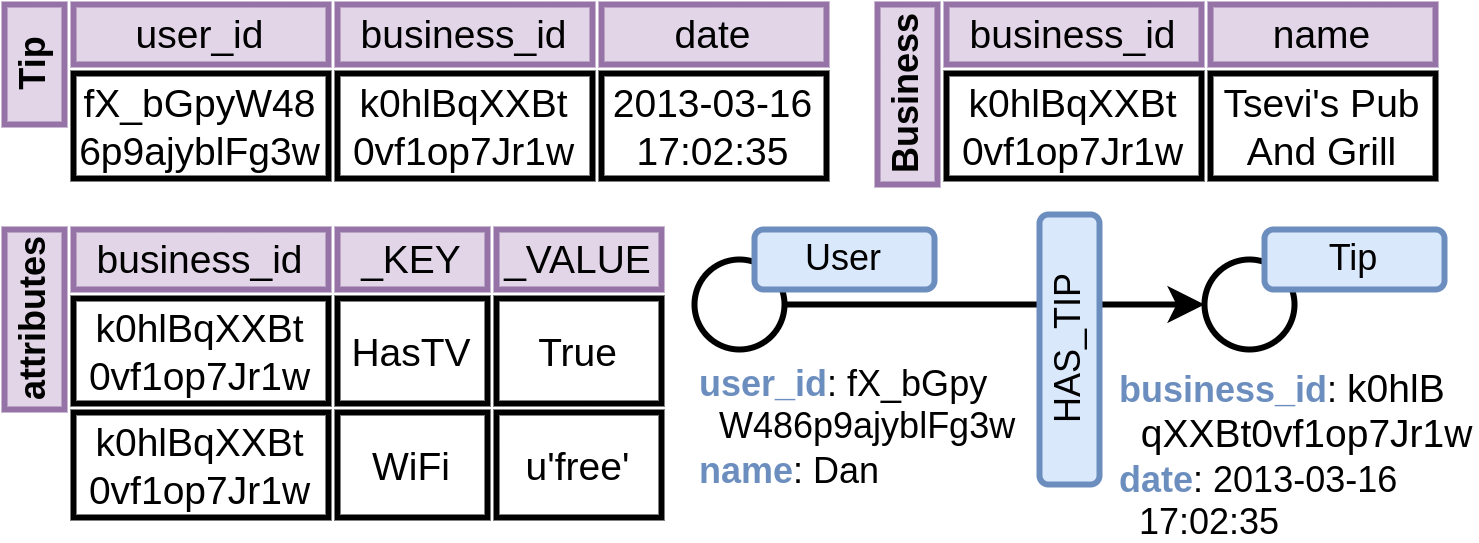
\includegraphics[width=0.8\textwidth]{papers/edbt_2025/figures/data-final.png}
    \caption{Yelp dataset in the graph and relational model}
    \pLabel{figure:data-final}
\end{figure}

%In order to cover real-world use cases, we continuously tested our tool on realistic datasets. We have encountered several challenges, which we have addressed by adding new features. We will demonstrate them using the Yelp dataset as an example. 

\subsubsection{Initial Schema Category}

\textit{TransforMMer} first infers the \textit{initial schema category} $\mathbf{S_{ini}}$ depicted for the input data in Fig.~\pRef{figure:sc-initial}. 
As we can see, each original JSON document corresponds to one kind in the schema category, namely \textit{User}, \textit{Business}, and \textit{Tip}.

%The dataset contains several kinds. Let's focus on \textit{business}, \textit{user}, and \textit{tip}. Our tool infers the schema of each kind, which is depicted in Fig.~\pRef{figure:sc-initial}.

\begin{figure}[ht]
    \centering
    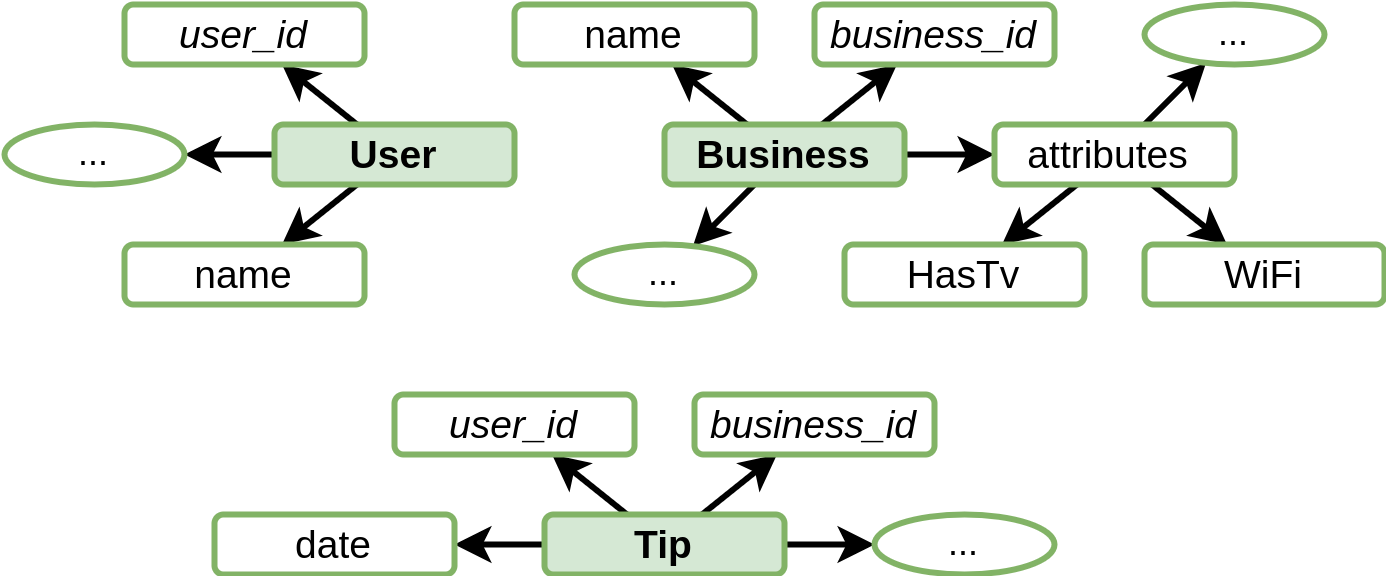
\includegraphics[width=0.8\textwidth]{papers/edbt_2025/figures/sc-initial.png}
    \caption{Initial schema category $\mathbf{S_{ini}}$ inferred from the sample data in Fig.~\pRef{figure:data-initial}}
    \pLabel{figure:sc-initial}
\end{figure}

\subsubsection{Improved Schema Category}
As $\mathbf{S_{ini}}$ is very simple and even incorrect, \textit{TransforMMer} enables its improvements. During the process of inference of $\mathbf{S_{ini}}$, it also infers a list of candidates for basic integrity constraints (identifiers and references), clustering, or recursion. The user can confirm or refuse them or add his/her suggestions to create an improved schema category $\mathbf{S_{imp}}$.

\paragraph{Identifiers}
First, we need an identifier for each kind to create a correct schema category. The inference process of \textit{TransforMMer} creates a list of simple properties that are candidate identifiers, i.e., they have a unique and compulsory value in each respective record. The user can select the correct ones from them. The candidates do not include composite identifiers, as finding all possible combinations would be too computationally expensive. However, the user can define composite identifiers manually.

In the sample $\mathbf{S_{ini}}$ in Fig.~\pRef{figure:sc-initial}, kind \textit{Business} has only one candidate identifier \textit{business\_id}, so we choose it as its identifier. %However, if we had used only a subset of the data, there might have been multiple candidate identifiers. In that case, we must rely on the domain knowledge to select the correct one. 
Kind \textit{User} also has only one candidate identifier \textit{user\_id}. Kind \textit{Tip} does not have any (simple) candidate identifier, so we create a composite identifier consisting of properties \textit{user\_id} and \textit{business\_id}. (The identifiers are depicted in Fig.~\pRef{figure:sc-final} in curly brackets in root nodes of the kinds.)

\paragraph{References}
Next, we can define references between the kinds to the respective identifiers. \textit{TransforMMer} also automatically infers candidates for the references (based on the inclusion of values of the referenced properties).

In the sample $\mathbf{S_{ini}}$ in Fig.~\pRef{figure:sc-initial}, we identify a reference from kind \textit{Tip} to kinds \textit{User} and \textit{Business} based on the values of properties \textit{user\_id} and \textit{business\_id}. The result is depicted in Fig.~\pRef{figure:sc-final}, where the two objects \textit{user\_id} were merged into one. The same happened for objects \textit{business\_id}. However, the primary identifier of kind \textit{Tip} is still the same; it is just represented by different schema morphisms.


\paragraph{Clustering of Properties}
Further improvements in the schema category involve the integration of various more complex constructs. One of them is replacing (huge) clusters of properties with maps. 
According to our analyses of real-world data, they may often contain multiple properties which have the same structure but different names (such as the property \textit{attributes} of kind \textit{Business} depicted in Fig.~\pRef{figure:sc-initial}). They make the schema unnecessarily complex, so \textit{TransforMMer} allows the user to transform them into a single set of key-value pairs. The user must just select all the properties to be represented as a map.  

The result is depicted in Fig.~\pRef{figure:sc-final}. As we can see, the direction of morphism between objects \textit{Business} and \textit{attributes} changed. This is because initially, the object \textit{attributes} corresponded to a complex property containing all the attributes, but now, it represents an array of key-value pairs. So, the cardinality specified by the morphism changed, and the morphism had to be updated (for details, see~\citep{DBLP:journals/jbd/KoupilH22}).

\begin{figure}[ht]
    \centering
    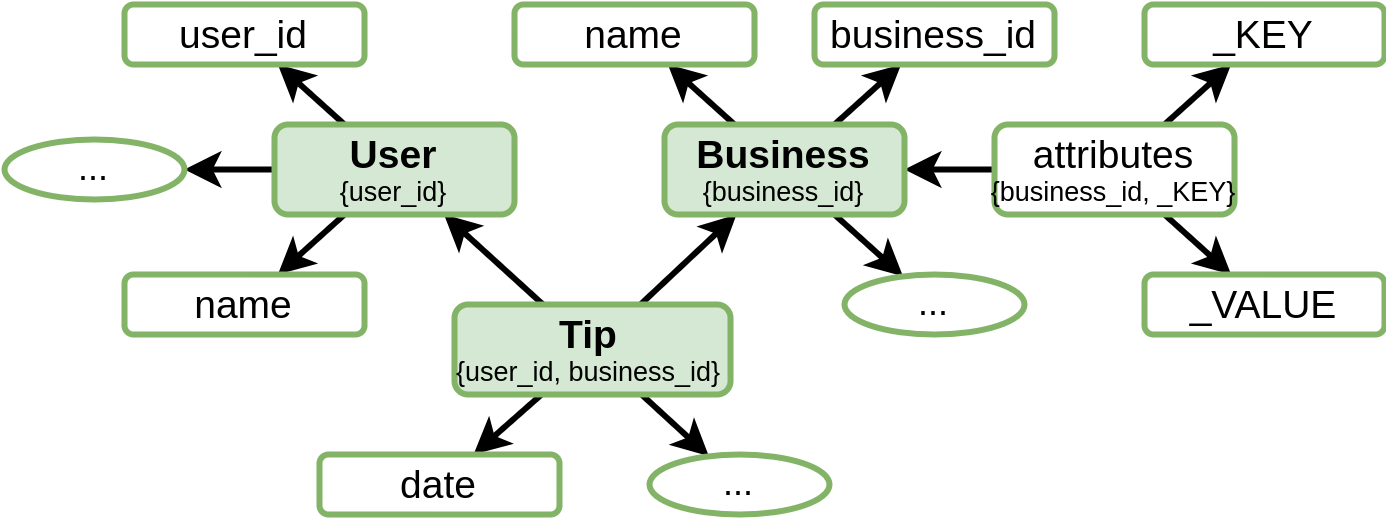
\includegraphics[width=0.8\textwidth]{papers/edbt_2025/figures/sc-final.png}
    \caption{The improved schema category $\mathbf{S_{imp}}$ of the Yelp data containing identifiers, a reference, and a map of properties}
    \pLabel{figure:sc-final}
\end{figure}

%Some datasets also use identifiers as property keys (e.g., UNESCO\footnotei{\url{https://ich.unesco.org/en/open-access-to-dive-data-01218}}){.} This is especially unfortunate because there is an arbitrary number of them (contrary to the large, but still manageable amount of business attributes in the Yelp dataset). The tool can handle it using the previous approach, but we are working on a better solution that would allow the users to define a pattern instead of manually selecting all the keys.

\paragraph{Recursion}
Similarly to clustering of properties, i.e., generally discovering a repeating pattern, we can also identify the recursion, i.e., a pattern occurring not within the same parent property but mutually nested. For example, consider a complex property \textit{comment} consisting of properties \textit{author}, \textit{content}, and \textit{replies}, where property \textit{replies} is an array of properties \textit{comment}. Such structure can be repeated in the inferred schema as many times as is the maximum depth of recursion in the source data.

We can significantly simplify this schema by defining a pattern for the property \textit{comment}. \textit{TransforMMer} then creates only a single complex property for each unique property in the pattern and a morphism from property \textit{replies} to property \textit{comment}. Thus, the resulting schema category contains a cycle, allowing infinite recursion. An example of such a transformation is depicted in Fig.~\pRef{figure:recursion}, which simultaneously provides sample screenshots of \textit{TransforMMer}.

\begin{figure}[h!]
%    \centering
%    \begin{minipage}{0.58\textwidth}
        \centering
        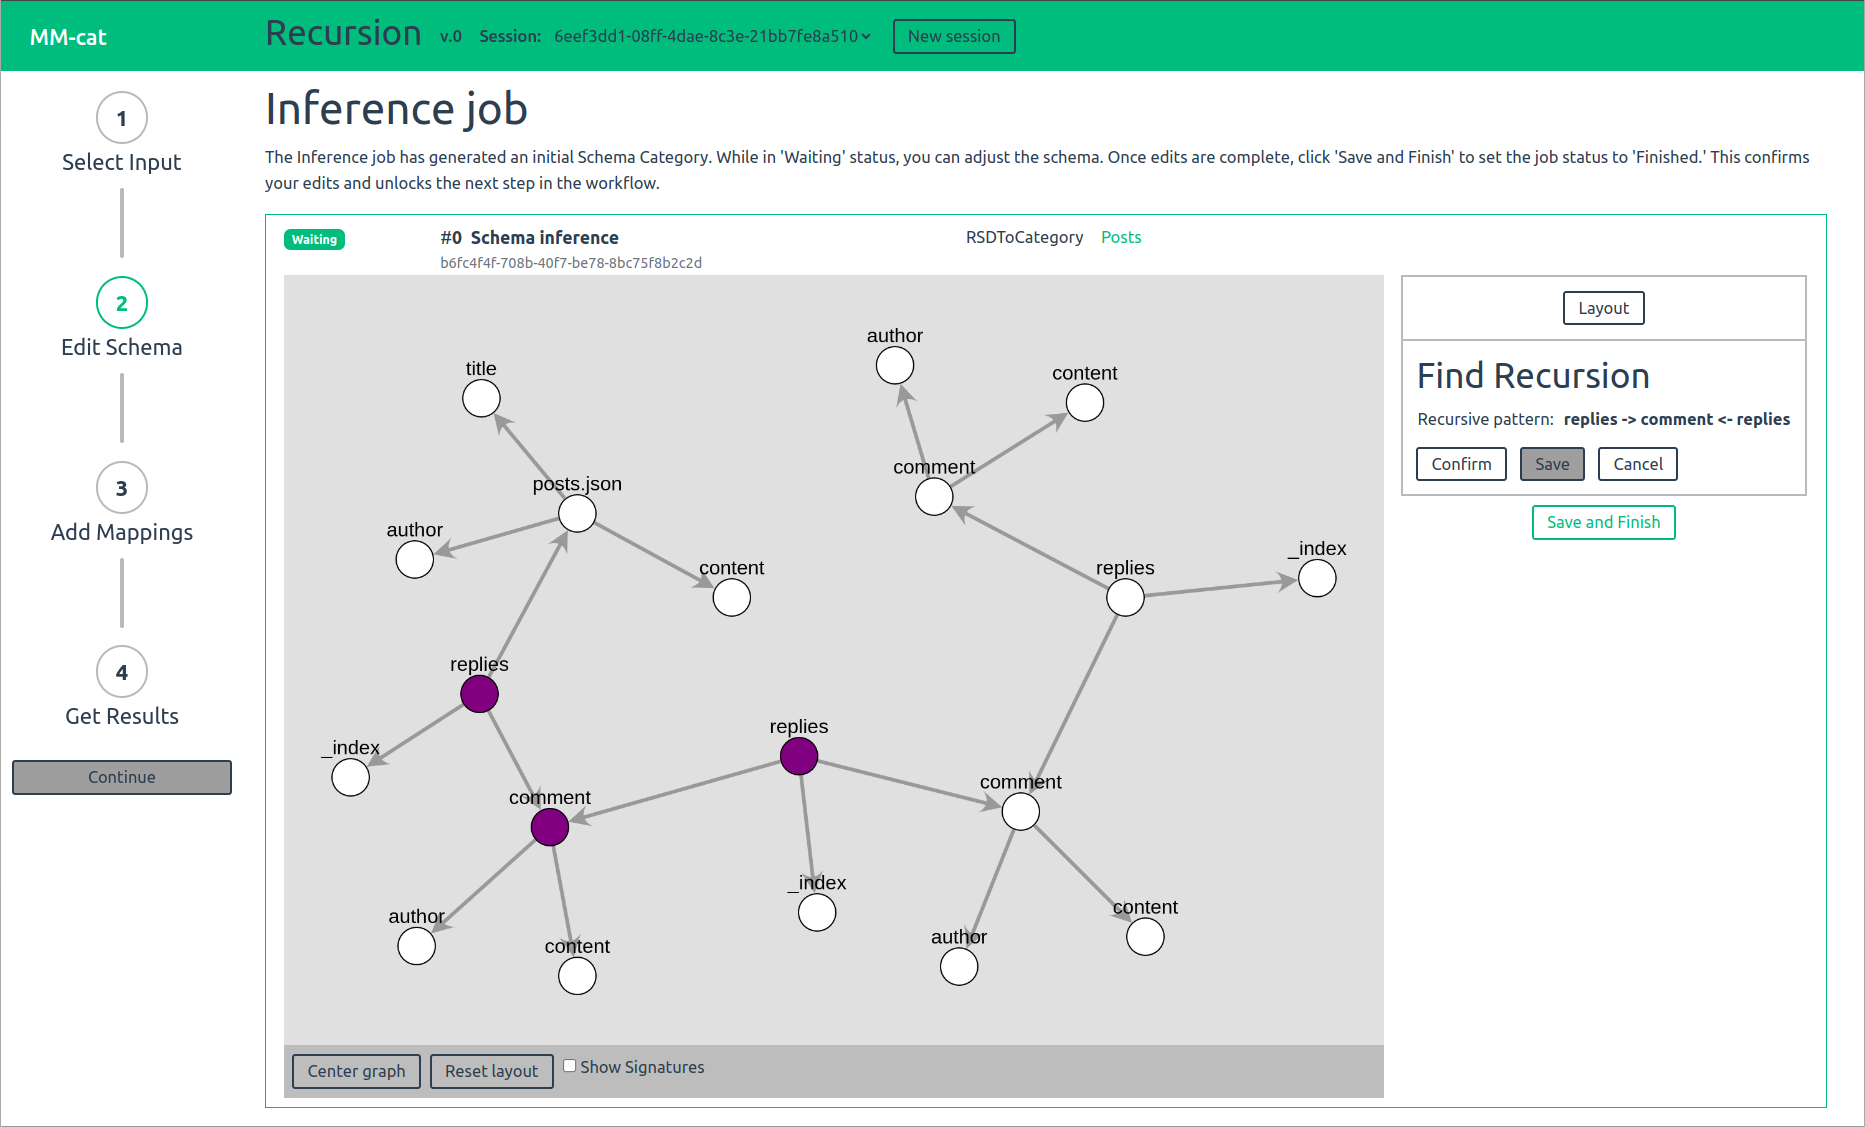
\includegraphics[width=\textwidth]{papers/edbt_2025/figures/recursion-initial-novalue.png}
%    \end{minipage}%
%    \begin{minipage}{0.42\textwidth}
%        \centering
        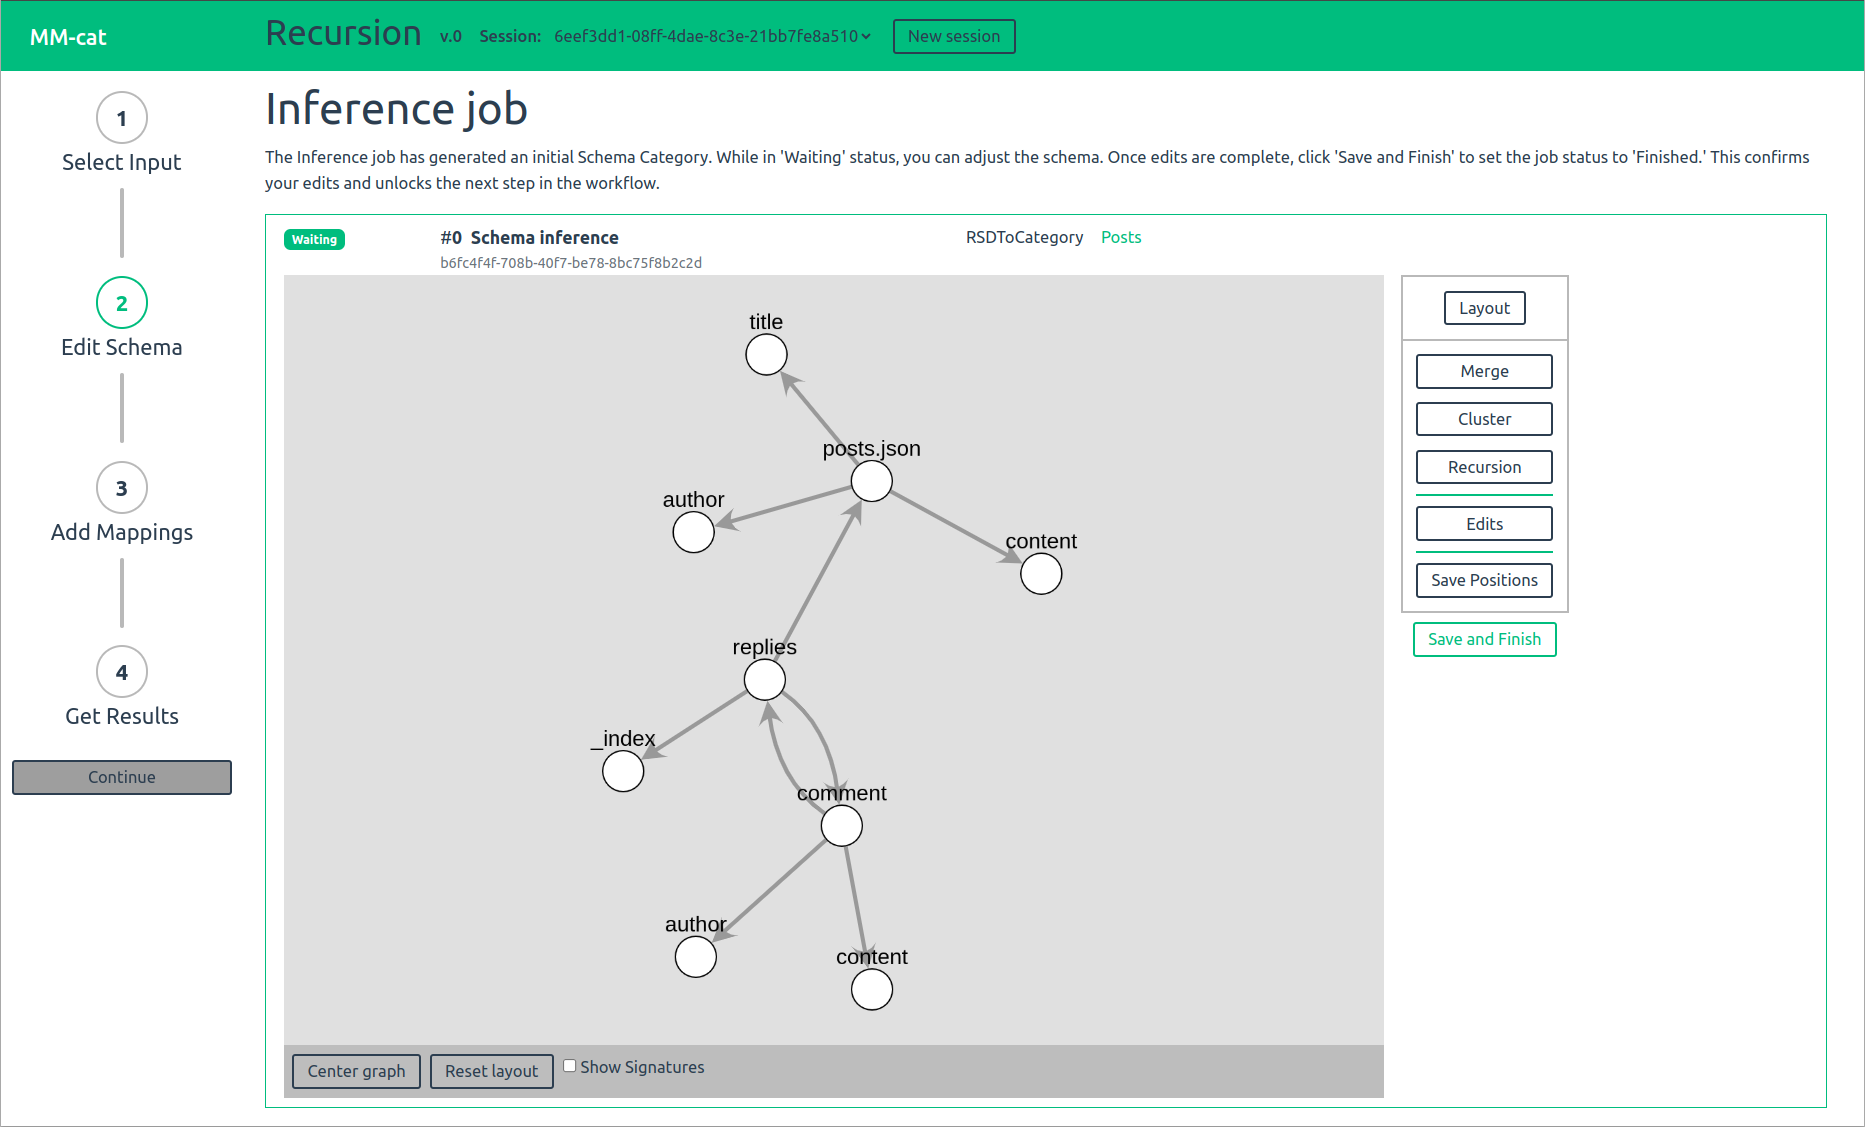
\includegraphics[width=\textwidth]{papers/edbt_2025/figures/recursion-final-wide-novalue.png}
%    \end{minipage}
    \caption{Screenshot of \textit{TransforMMer} before and after the elimination of a recursive structure}
    \pLabel{figure:recursion}
\end{figure}

\subsubsection{Mapping Modification}
Having the final improved schema category $\mathbf{S_{imp}}$ (see Fig.~\pRef{figure:sc-final}), the user can now define its new mapping. As depicted in Fig.~\pRef{figure:sc-multi}, for example, the original document model (green) can be entirely discarded, and instead of it, the user may define four new kinds. Kind \textit{User} is mapped to the graph model (blue), where each user represents a node in the graph, and edges represent mutual friendship. Kinds \textit{Business}, \textit{Tip}, and \textit{attributes} are mapped to the relational model (purple), i.e., tables. Considering the relational model without arrays, the kind \textit{attribues} had to be established. The output data are depicted in Fig.~\pRef{figure:data-final}.

\begin{figure}[h!]
    \centering
    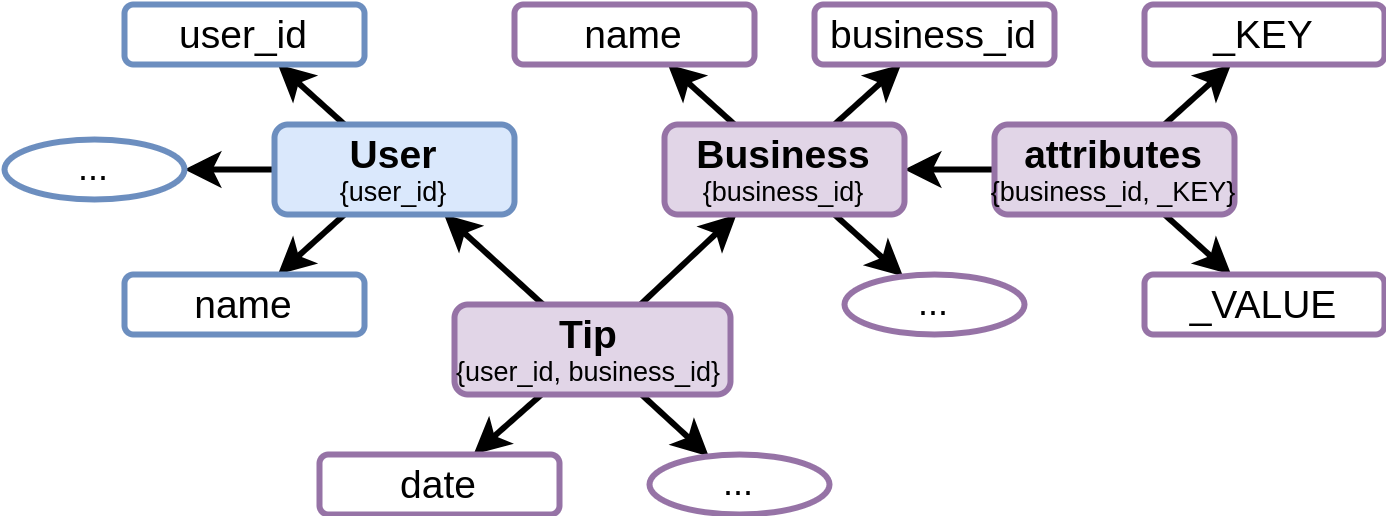
\includegraphics[width=0.8\textwidth]{papers/edbt_2025/figures/sc-multi.png}
    \caption{$\mathbf{S_{imp}}$ of the Yelp data re-mapped to the graph (blue) and relational (purple) model to represent data in Fig.~\pRef{figure:data-final}}
    \pLabel{figure:sc-multi}
\end{figure}

\subsection{Workflow}
The whole process of transforming the input (single- or multi-model) data to required multi-model data is depicted in Fig.~\pRef{figure:workflow}.

\begin{figure}[h!]
    \centering
    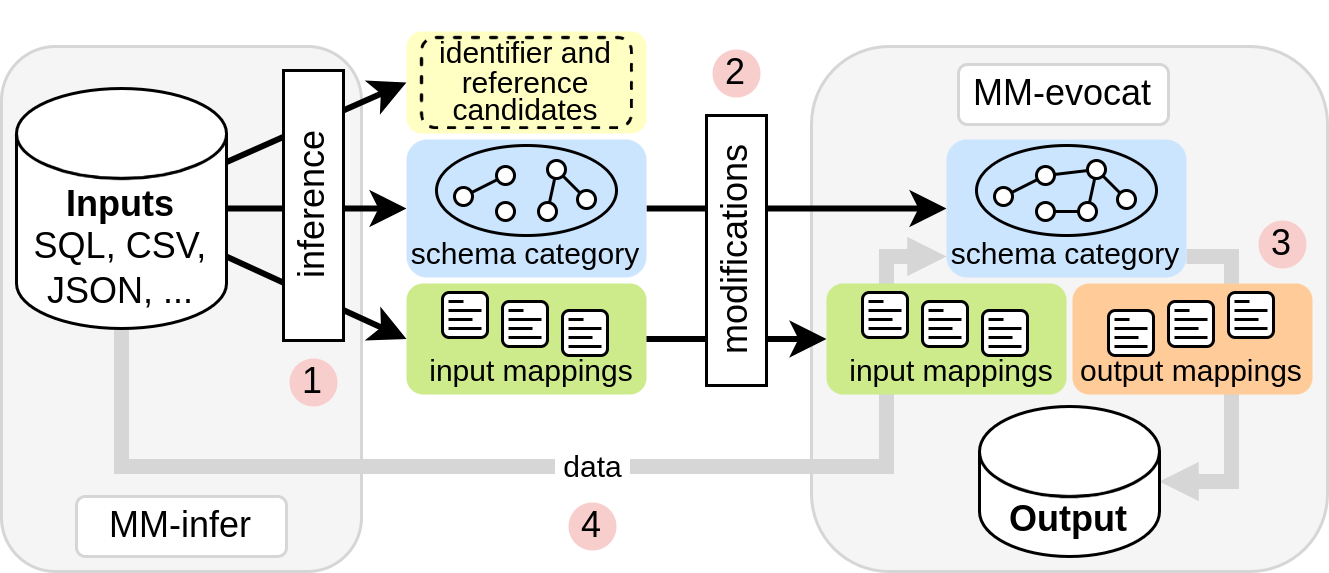
\includegraphics[width=\textwidth]{papers/edbt_2025/figures/workflow.png}
    \caption{The workflow of \textit{TransforMMer}}
    \pLabel{figure:workflow}
\end{figure}

\paragraph{Step 1}
First, the users need to specify input data sources. \textit{TransforMMer} supports the input from a file system, a DBMS, or their combination. It then infers the schema of each kind (table, collection, etc.) in the data sources. The output of this step is $\mathbf{S_{ini}}$ and its mapping to the logical structures of the original data. The algorithm also infers candidates for identifiers, references between the kinds, and repeating patterns. %An example of such SC is shown in Fig.~\pRef{figure:sc-initial}.

\paragraph{Step 2}
$\mathbf{S_{ini}}$ is improved by interacting with the user, i.e. $\mathbf{S_{imp}}$ is created. The user can specify identifiers, references, and repeating patterns to be merged from the candidate set or his/her own.
%The inferred SC can not be used directly. In order to produce multi-model data, the users need to specify identifiers of the kinds and references between them. This is done semi-automatically (see section \pRef{section:real-data}). The results are shown in Fig.~\pRef{figure:sc-final}.
The user can also further modify the schema category, e.g., by grouping a set of properties into a new property or deleting a property. With every change, \textit{TransforMMer} automatically updates the mappings. 


\paragraph{Step 3}
$\mathbf{S_{imp}}$ is mapped to the new requested combination of models. The user selects parts of the schema category and specifies the requested, possibly overlapping mapping (e.g., by modifying an existing one or creating a new one from scratch). \textit{TransforMMer} ensures all the respective modifications.

%For example, the original data was in JSON files (i.e., document model). However, we want to transform it into a combination of PostgreSQL (relational) and Neo4j (graph) databases (see Fig.~\pRef{figure:sc-multi}).

\paragraph{Step 4}
\textit{TransforMMer} loads the original data according to the input mappings into an in-memory categorical representation and then stores it according to the new user-specified mappings into the output. It can be stored in a specified file system or a DBMS.


\subsection{Architecture}
As mentioned in the introduction, \textit{TransforMMer} leverages selected members of our toolset for multi-model data management, namely \textit{MM-infer}~\citep{mm_infer} for categorical schema inference, \textit{MM-evocat}~\citep{mm_evocat} for schema modifications, and \textit{MM-cat}~\citep{mm_cat} (now a part of \textit{MM-evocat}) for schema modelling and data transformations. Fig.~\pRef{figure:workflow} also indicates their integration in \textit{TransforMMer}. \textit{TransforMMer} consists of the backend (written in Java), which contains all the algorithms, and a single-page client (written in Vue), which provides the user interface. The code repository is available at GitHub\footnotei{\url{https://github.com/mmcatdb/mmcat}}{.} And a demo is also available\footnotei{\url{https://demo.mmcatdb.com}}{.} Lastly, we have a short video tutorial\footnotei{\url{https://www.youtube.com/watch?v=Aiw815OaAb4}}{.}

All of the algorithms mentioned above use abstract wrappers, which provide a unified interface to the data sources instead of working with them directly. This allows us to easily add support for new data sources by implementing a new wrapper. For now, we support PostgreSQL, MongoDB, Neo4j (i.e., representatives of the relational, document, and graph model), CSV and JSON files (i.e., the most common file formats).

Because the users might want to work with large datasets, all processes are implemented as asynchronous jobs. %The users can start the jobs and then return later to check the results.

\subsection{Dataset Repository}
As a proof of concept, we have used \textit{TransforMMer} to generate a repository\footnote{\url{https://dare.mmcatdb.com}} of popular multi-model datasets (to be gradually extended). The current datasets involve, e.g., the Yelp dataset, the IMDb dataset\footnotei{\url{https://developer.imdb.com/non-commercial-datasets/}}{,} or the dataset of NASA open-source code projects\footnotei{\url{https://data.nasa.gov/Software/NASA-open-source-code-projects-with-A-I-generated-/3efg-u4v8/about-data}}{.} In the next steps, we want to extend the repository with the popular datasets and their variations and using a comparative survey demonstrate the wide usability of \textit{TransforMMer} for comparing multi-model databases.
